% !TEX root = ../main.tex
%
\chapter{Technical Implementation}
\label{sec:system}

\section{System Architecture}
\label{sec:system:architecture}

The architectural design adheres to the conventional client-server paradigm, with the server acting as a wrapper for the Nerfstudio Command Line Interface (CLI) and the client as a web application.
The service is responsible for handling incoming requests from the client and translating them into commands that the Nerfstudio CLI could understand.
Requests from the client are transmitted to the service via HTTP.
In the event of an asynchronous operation, the server updates the client via WebSockets. \fref{sec:system:architecture}.

\begin{figure}[htb]
	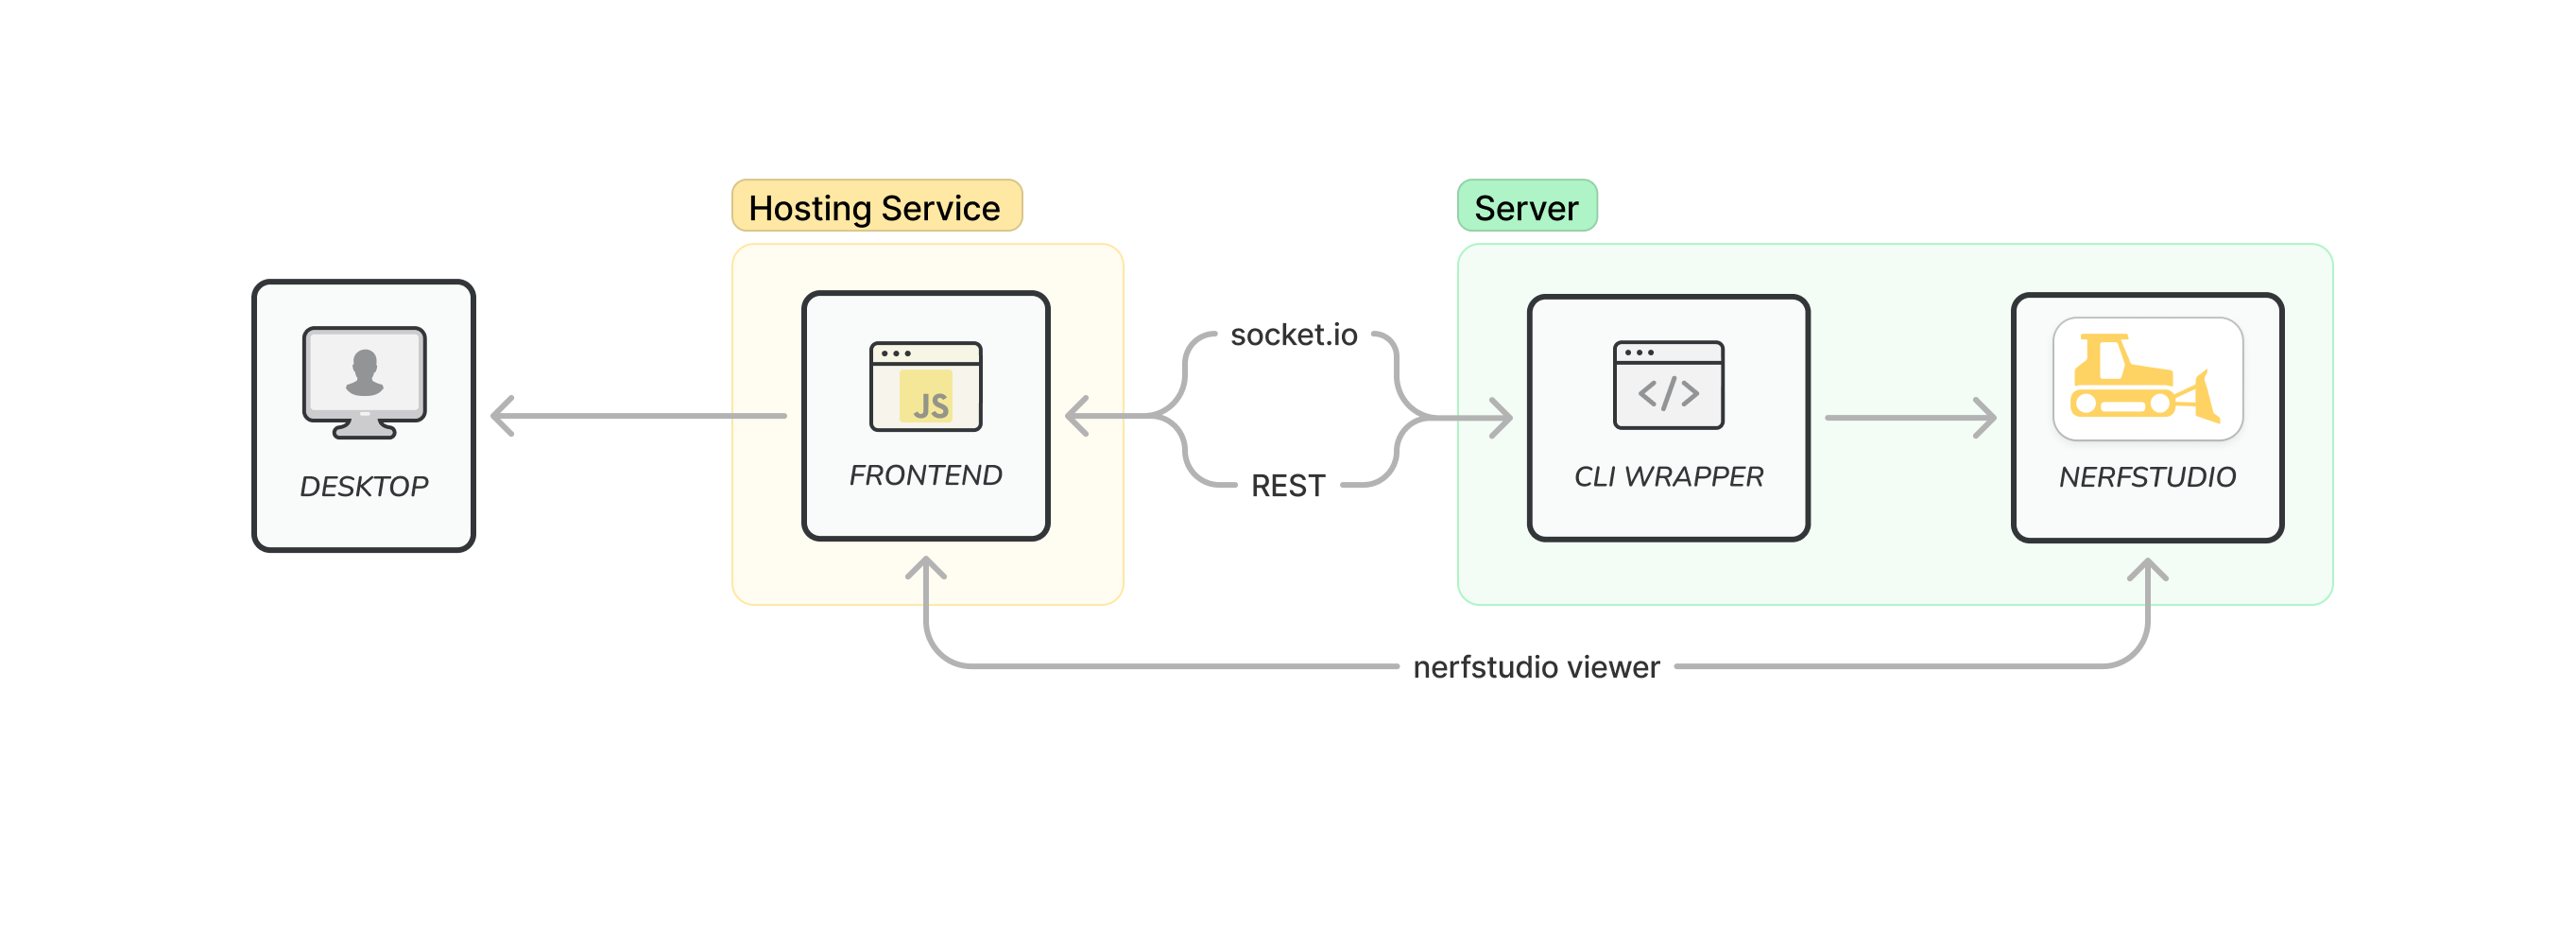
\includegraphics[width=\textwidth]{figures/architecture-1.png}
	\caption{System Architecture Overview. The client communicates with the server, which in turn interacts with the nerfstudio CLI.}
	\label{fig:system:example2}
\end{figure}

In case of the prototype, all components were integrated into a single Docker \cite{noauthor_docker_2022} container and deployed as a single unit.
This approach made use of the pre-configured container provided by Nerfstudio, facilitating a rapid and straightforward deployment.
All source code is available in the project's GitHub repository \cite{von_briesen_simplify-nerf_2024} and pre-built Docker images are hosted on Docker Hub \cite{von_briesen_eduardvbsimplify-nerf_nodate}.

\section{Frontend Development} 
\label{sec:system:frontend}

The frontend is built with React \cite{noauthor_react_nodate}, chosen for its popularity and strong support in web application development.
Vite \cite{noauthor_vite_nodate} serves as the build tool, offering a fast and efficient development experience.
For styling, Tailwind CSS \cite{noauthor_tailwind_2020}, a utility-first CSS framework, provides a set of predefined classes to style components efficiently.
Additionally, the daisyUI \cite{noauthor_daisyui_nodate} component library supplies pre-styled components, facilitating rapid UI construction.

\subsubsection{Extensibility}

Extensibility was a key consideration during the development of the frontend, given that the underlying Nerfstudio CLI is in itself extensible.
All parameters for processing and training a NeRF model are configurable using JSON or strongly typed TypeScript objects (see Listing \ref{lst:config}).

\begin{figure}[htb]
\begin{lstlisting}[style=ES6, caption=Minimal parameter configuration for 'Steps Per Save' input., label=lst:config]
const stepsPerSave: NumberInput = {
	name: "stepsPerSave",
	label: "Steps Per Save",
	tooltip: "Number of steps between each save of the model.",
	inputType: "number",
	defaultValue: 1000,
};
\end{lstlisting}
\end{figure}

The current input types supported are \texttt{number}, \texttt{select}, and \texttt{boolean}. 
This covers all relevant parameters, but new types can be added by extending the configuration object. 
It is also possible to define dependent parameters that are only shown when a certain condition is met. 
Furthermore, images can be added to illustrate the effect of a parameter, providing additional context to the user.

Additionally, filters and presets may be configured by specifying an array of the names of the parameters that should be included in the filter or preset.
This is currently employed to narrow down the displayed options and expand them when activating advanced settings. 
The complete configuration may be found in the \texttt{frontend/src/config} folder within the codebase.

\subsubsection{Nerfstudio Viewer Integration}

The Nerfstudio viewer is constructed using Viser \cite{noauthor_nerfstudio-projectviser_2024}, a Python library for developing 3D visualizations.
This approach presented certain limitations in integrating it into the frontend, as it is not straightforward to embed a Python application directly into a web application.
To circumvent this issue, the viewer is hosted by Nerfstudio and embedded into the frontend using an iframe.
This included some simple styling changes to enhance the viewer's integration into the frontend.
Additionally, modifications were implemented to enhance the user experience.
The viewer contained several interactions where it was necessary for the user to copy console commands, which were to be used in the CLI.
These interactions are replaced with buttons that send a request to the server to execute the command instead. 
These modifications are applied at the build-time of the container by applying a patch to the Nerfstudio source code of the base image.

The main shortcoming of this approach is that the frontend is unaware of the state of the viewer, and cannot update the UI based on actions triggered in the viewer.
Instead, it must rely on periodic polling of the server to obtain the current status of rendering processes, which is then used to provide feedback to the user.

\section{Backend Development}
\label{sec:system:backend}

The backend was constructed using tRPC \cite{noauthor_trpc_nodate}, a framework for developing type-safe APIs in TypeScript.
This type-safety proved beneficial in the construction of the API, as Nerfstudio endpoints necessitate a specific set of parameters of various types, which could be readily defined using TypeScript and reused in the frontend.

It is often the case that processes can take several minutes to complete.
In such instances, it is important that the user is able to see the progress of these operations.
tRPC implements subscriptions, which allows the client to subscribe to an event and receive updates when that event occurs.
This is used for any long-running operations such as pre-processing or training a NeRF model (see Listing \ref{lst:trpc}).


\begin{figure}[htb]
\begin{lstlisting}[style=ES6, caption=Example tRPC endpoint for Pre-Processing returning a subscription., label=lst:trpc]
export const nerfstudioRouter = router({
	process: publicProcedure
		.input(
			z.object({
				project: z.string(),
				dataType: z.enum(["images", "video"]),
				...
			}),
		)
		.subscription(({ input }) => {
			return observable<{message: string}>((emit) => {
				const args = ...
				const process = spawn("ns-process-data", args, {
          cwd: path.join(WORKSPACE, input.project),
        })
				process.stdout.on("data", (data: any) => {
					emit.next({message: data.toString()});
				});
			});
		})
});
\end{lstlisting}
\end{figure}

additional endpoints were implemented using Express \cite{noauthor_express_nodate}, including the file upload and render endpoints, due to limitations in tRPC discussed in Section \ref{sec:system:challenges}.

All project related data is stored in a workspace directory, which is mounted as a volume in the Docker container.
This allows for the data to persist between container restarts, and for the user to access the data outside of the container.

\section{Challenges and Solutions}
\label{sec:system:challenges}

\subsection*{Limitations of tRPC}

Although tRPC is a highly effective tool for developing APIs, with seamless integration into the frontend, it is not without its limitations.
It lacks support for \texttt{multipart/form-data} file uploads, which are necessary for uploading images and videos.
This issue was addressed by implementing a distinct endpoint utilizing Express, which is employed for the purpose of uploading files to the server.

Additionally, the manner in which tRPC handles subscriptions is not optimal for the execution of lengthy processes.
In the event of a client disconnect, the subscription is lost, and the client will lose the context for incoming events.
An improved solution would utilize a standard WebSocket connection, with the events containing the state necessary for the client to properly update the UI.

tRPC lacks a client for Python, which is required when processes are initiated from the Nerfstudio viewer.
This necessitated the implementation of an additional distinct endpoint utilizing Express, which is invoked by the viewer to render the NeRF model.
These limitations could be mitigated by the use of a more general-purpose framework, such as Express.

\subsection*{Working with the nerfstudio CLI}

The implementation of the prototype using the nerfstudio CLI offered a useful layer of abstraction, enabling rapid development without the necessity to concern oneself with the underlying implementation details of a vast codebase.
However, this abstraction comes at the cost of flexibility and the overall complexity of the system.

The CLI is constructed using tyro \cite{yi_tyro_nodate}, a tool for the creation of command line interfaces in Python utilising configuration objects.
Efforts were made to translate the configuration objects into TypeScript objects that could be employed throughout the project.
This would facilitate a more seamless integration of the CLI.
Regrettably, this was not feasible, as the configuration objects are not readily serializable and would necessitate a significant amount of additional work to implement.
Consequently, the implemented solution is reliant on manually constructing the commands based on documentation, which is error-prone and not particularly maintainable.
\section{Future Directions}
\label{sec:system:future}

\subsection*{Improved CLI Integration}

As outlined above, the approach of wrapping the Nerfstudio CLI with a custom API has some limitations.
A more integrated and robust solution would be to built within the Nerfstudio codebase itself.
It is conceivable that the existing configuration object, utilized for the CLI, could be repurposed to construct a REST API.
This would facilitate a more seamless integration of the CLI into the frontend, and would allow for greater flexibility in the future.
Furthermore, this approach would reduce the overall complexity of the system, as it would not require the use of a separate server to handle requests.

\subsection*{Improved Viewer Integration}

The current approach of embedding the viewer in an iframe is not optimal.
The Nerfstudio viewer in versions 0.3.4 and earlier was constructed using React with a direct integration of Viser.
In its first major release, nerfstudio rewrote the viewer in Python, thereby eliminating the React integration.

The reconstruction of this project's frontend with a framework such as Viser would be severely constrained in terms of features and flexibility.
A more optimal solution would be to integrate Viser into the front end, analogous to the original nerfstudio viewer.
Such an integration would facilitate a more seamless interaction between the frontend and the viewer, thereby enhancing the overall user experience.
The re-use of UI elements would ensure a consistent look and feel, while the frontend could react to events triggered in the viewer.